\documentclass[final]{fhnwreport}       %[mode] = draft or final
                                        %{class} = fhnwreport, article, 
                                        %          report, book, beamer, standalone
\input{header}			                %loads all packages, definitions and settings											
\title{Fachbericht}  		        %Project Title
\author{Team 1}      				    %Document Type => Technical Report, ...
\date{\today}          				   %Place and Date

\begin{document}

%%---TITLEPAGE---------------------------------------------------------------------------------
\thispagestyle{empty}
%	\ohead{\includegraphics[scale=0.5]{Bilder/Logo_FHNW.jpg}}
	\begin{figure}
		 \vspace*{-\topskip}\vspace*{-\headsep}
		\includegraphics[scale=1]{graphics/fhnw_ht_logo_de.pdf}
	\end{figure}
	\begin{center}
		\vspace*{2cm}
		{\huge{\textbf{digitales Theremin}}}\\
		\vspace*{0.2cm}
		{\huge{\textbf{\thetitle}}}\\
		\vspace*{0.5cm}
		
		{\scshape\Large Projekt 5\\} \Large{\today}
		\vfill
		\begin{normalsize}
			{\begin{tabbing}
					\textbf{Auftraggeber:} \hspace{5cm}\= Prof. Dr. Hanspeter Schmid\\
					
					\\[0.8cm]
					\textbf{Betreuung:} 
					\>Prof. Dr. Hanspeter Schmid\\
					\>Herr Prof. Karl Schenk\\


					\\[0.8cm]
					\textbf{Team:} \>Andreas Frei \\ \>Dennis Aeschbacher \\ 

					\\[0.8cm]
					\textbf{Studiengang:} \>Elektro- und Informationstechnik
					\\[0.8cm]	\textbf{Semester:} \>Herbstsemester 2019
			\end{tabbing}}
		\end{normalsize}
		\vfill
	\end{center}
\clearpage
			
%%---ABSTRACT----------------------------------------------------------------------------
\selectlanguage{english}				%ngerman or english
\thispagestyle{empty}
\begin{abstract}
% Description aim/objective
\noindent This project was a continuation on the work on a Theremin that mainly operates on digital hardware. Unlike the original device, which solely used analog electronics. The device is supposed to be used in presentations for trade fairs by the Institute for Sensors and Electronics ISE. As such the device should be built in an appealing housing. Moreover the device should have other additional functionality that helps the player to use the instrument more easily.
% Method
The digital hardware was implemented in VHDL on the developer board DE1-SoC from terasIC with a Cyclone V FPGA from Intel. The sole analog component implemented were the oscillators that control the pitch and volume by use of two antennae and the codec, wich converts the audio data for use on a loudspeaker. 
% Results
The pitch and volume of the instrument can be changed by the two antennae like a usual theremin. To adjust settings the theremin has a touchscreen display that is controlled by the Nios system, that was implemented. The theremin has two functionalities, that help the player use the instrument more easily. First the glissando effect, wich corrects the pitch to the closest musical note. Second the pitch display, wich displays the closest musical note the player ist playing at and the deviation that the player is causing.
% Conclusion
In conclusion it can be said, that the theremin is ready for any trade fairs that will come.


\end{abstract}	



%%---TABLE OF CONTENTS-------------------------------------------------------------------
\pagenumbering{Roman}		
\selectlanguage{ngerman}				%ngerman or english
\tableofcontents
\clearpage

%%---TEXT--------------------------------------------------------------------------------
\pagenumbering{arabic}
\clearpage
\section{Einleitung}\label{sec:Einleitung}
Das Theremin kennen heutzutage nur wenige Leute, obwohl es das erste elektronische Instrument war. Es wurde 1920 von dem Russen Lev Sergejewitsch Termen, welcher sich später zu Leon Theremin umbenennen liess, erfunden \cite{Theremin_h}. Personen die regelmässig Filme schauen, haben die Musik welche mit einem Theremin gemacht wird bestimmt schon einmal gehört. Ein Beispiel dafür ist Ghostbusters, wo das Theremin oft im Hintergrund zu hören ist. Zudem ist das Theremin in einigen Science-Fiction-Filmen und Horrorfilmen zu hören \cite{Goast_m}. Das Theremin wird ohne es zu berühren gespielt, indem man mit den Händen die Distanz zu zwei Antennen ändert. Dies führt zu Veränderung der Tonhöhe und Lautstärke.

Im Projekt 5 und 6 soll nun ein solches Instrument entwickelt werden. Mit dem Unterschied, dass das sonst analoge Instrument digital aufgebaut werden soll. Dabei soll es auf einem Field Programmable Gate Array (FPGA) implementiert werden. Später soll das Theremin als Messeobjekt für das Institut für Sensorik und Elektronik ISE verwendet werden. Im Rahmen des Projekt 5 wurde die Tonhöhenantenne des Theremin realisiert. Dazu wurde die Antenne zusammen mit dem Antennenoszillator analog beibehalten. Die restlichen Komponenten wurden in VHDL realisiert. Das Resultat wurde auf dem DE1-SoC Board von terasIC mit einem Cyclone V FPGA von Intel getestet.

Der folgende Fachbericht beginnt mit dem Kapitel \ref{sec:Technische Grundlagen} Technische Grundlagen.In der ersten Hälfte des Kapitel wird erklärt wie ein analoges Theremin funktioniert und welche Komponenten ein Theremin ausmachen. In der zweiten Hälfte werden digitale Lösungsansätze besprochen. Anschliessend wird im Kapitel \ref{sec:Realisierung} Realisierung beschrieben wie die Komponenten realisiert wurden. Im Kapitel \ref{sec:Validierung} Validierung wird als erstes auf die Inbetriebnahme des Antennenoszillators eingegangen. Als nächstes werden die Simulationen des VHDL Codes erläutert. Im letzten Abschnitt wird auf die Inbetriebnahme des VHDL Codes auf dem DE1-SoC Board Bezug genommen.


\todo{Erklärung zu Glissando und Anzeige Spielgenauigkeit}




\pagebreak

	
\clearpage
\section{Technische Grundlagen}\label{sec:Technische Grundlagen}
In diesem Kapitel ist als erstes erklärt wie ein analoges Theremin funktioniert um ein Verständnis für dessen Funktionsweise zu gewinnen. Anschliessend folgt ein kleiner Abschnitt zur Musiktheorie. Zuletzt werden verschiedene Algorithmen erklärt, welche im digitalen Theremin eingesetzt wurden.
	\subsection{Analoges Theremin}\label{subsec:Theremin_analog}
Das klassische Theremin besitzt zwei Antennen. Der Spieler kann über die senkrecht angebrachte Antenne  die  Tonhöhe beeinflussen. Mit der waagrechten Antenne regelt der Spieler die Lautstärke. Eine typische Eigenschaft des Theremins ist, dass der Ton des Theremins in einem weiten Frequenzbereich kontinuierlich veränderbar ist. Das Theremin kann daher alle Frequenzen in einem Bereich spielen, im Gegensatz zu den meisten anderen Instrumenten.

Der Spieler spielt das Theremin durch verstimmen der Oszillatoren über die Antennen.
Die Hand des Spielers verändert über die jeweilige Antenne die Schwingfrequenz des Tonhöhen- und Lautstärkenoszillators. Dabei wird der kapazitive Anteil des LC-Schwingkreises beeinflusst, was eine Änderung der Schwingfrequenz zur Folge hat. 
Die Frequenz dieser Oszillatoren ist jedoch weit über dem hörbaren Bereich (zwischen \SI{100}{kHz} bis \SI{1}{MHz}). Mit Hilfe eines Mischers und einem Referenzoszillator wird die Frequenzdifferenz des Tonhöhenoszillators hörbar gemacht und danach verstärkt\cite{Franzis}. Der Lautstärkepegel ergibt sich durch die Verwendung eines Bandpassfilters und eines nachfolgenden Hüllkurvendetektors. Die Abbildung \ref{img:Blockschaltbild_analog} gibt einen Überblick über die Schaltungskomponenten eines Theremins. Die einzelnen Schaltungsteile sind im folgenden Teil genauer erklärt.

\begin{figure}[h]
	\centering
	\includegraphics[width=0.8\textwidth]{Blockschaltbild_analog.pdf}
	\caption{Blockschaltbild eines analogen Theremins}
	\label{img:Blockschaltbild_analog}
\end{figure}

\paragraph{Tonhöhenoszillator und Tonhöhenantenne}\mbox{}\\

Die Tonhöhenantenne ist ein Metallrohr, welches mit dem Tonhöhenoszillator verbunden ist.
Der Spieler kann über die Distanz seiner Hand zur Antenne die Frequenz des Tonhöhenoszillator verändern. Die über die Antenne zu erreichende Kapazitätsänderung ist sehr gering. Diese liegt im Picofarad Bereich \cite{physik_theremin}. Die Grundfrequenz des Tonhöhenoszillators muss weit über dem hörbaren Bereich liegen, damit eine genügend grosse Frequenzänderung entsteht.

\paragraph{Lautstärkenoszillator und Lautstärkenantenne}\mbox{}\\ 

Die Lautstärkenantenne ist wie die Tonhöhenantenne ein Metallrohr, welches mit dem Lautstärkenoszillator verbunden ist. Die durch den Spieler beeinflusste Frequenzänderung wandelt ein Hüllkurvendetektor in eine Spannung um. Diese Spannung dient dem Verstärker als Steuergrösse, um das Audio Signal zu verstärken. \cite{Franzis}. 

\paragraph{Mischer und Referenzoszillator}\mbox{}\\ 
\\Die erzeugte Frequenz der Tonhöhenantenne liegt weit über dem vom Menschen hörbaren Bereich. Der Mischer multipliziert die Signale des Referenzoszillators und des Tonhöhenoszillators wie in Formel \ref{equ:mischer}. $A_1\sin(\omega_1t)$ entspricht dem Signal des Referenzoszillators und $A_2\sin(\omega_2t)$ dem Signal des Tonhöhenoszillators.

\begin{equation}
V_{out} = A_{1}A_{2} \sin(\omega_{1}t)   \sin(\omega_{2}t) 
\label{equ:mischer}
\end{equation}

$V_{out}$ kann durch Additionstheoreme umgeformt werden. Dabei erhält man folgenden Ausdruck:

\begin{equation}
V_{out} = A/2[\cos((\omega_{1}-\omega_{2})t)  - \cos((\omega_{1}+\omega_{2})t) ]
\label{equ:mischer_trigo}
\end{equation}

Das Ausgangssignal $V_{out}$ hat zwei Frequenzkomponenten. Zum einen die Differenz der beiden Frequenzen, zum anderen die Summe der Frequenzen. Dabei ist bei dem Theremin nur die Differenz der Frequenzen von Interesse \cite{physik_theremin}.

Eine Kalibration des Theremins ist vor jedem Gebrauch nötig. Es könnte beispielsweise sein, dass die Differenz der Frequenz ausserhalb des hörbaren Bereiches liegt. Dazu stellt der Spieler beim klassischen Theremin mit Hilfe eines Trimmkondensators am Referenzoszillator die Differenzfrequenz auf \SI{0}{Hz} ein.

\paragraph{Tiefpassfilter}\mbox{}\\ 
\\Das Tiefpassfilter filtert die hochfrequente Komponente aus Formel \ref{equ:mischer_trigo} weg. Übrig bleibt die Differenz der Oszillatorfrequenzen. Dies ist der interessante Anteil des Mischprozesses, da er im hörbaren Bereich liegt.
\begin{equation}
V_{out} = A/2cos((\omega_{1}-\omega_{2})t) 
\label{equ:mischer_gefilt}
\end{equation}

\paragraph{Verstärker und  Lautsprecher}\mbox{}\\ 
\\Der Verstärker verstärkt das Ausgangssignal des Tiefpassfilters abhängig von der Spannung, welche vom Hüllkurvendetektor stammt.

	\subsection{digitales Theremin}\label{subsec:Theremin_digital}

Wie schon am Anfang dieses Kapitels angedeutet, werden in diesem zweiten Teil Möglichkeiten für den Aufbau des Theremins als ein digitales Instrument aufgezeigt.
\begin{figure}[h]
	\centering
	\includegraphics[width=0.7\textwidth]{Blockschaltbild_digital.pdf}
	\caption{Blockschaltbild digitales Theremin mit eingezeichneten Ausgängen.}
	\label{img:Blockschaltbild_digital}
\end{figure}

\paragraph{Antennenoszillator}\mbox{}\\
\\Um den Oszillator zur Änderung der Tonhöhe und der Lautstärke zu realisieren waren mehrere Optionen möglich. Diese wurden in der Projektklärung genauer verglichen (siehe Anhang). Schlussendlich wurde entschieden, dass dieser Teil des Theremins weiterhin analog bleiben soll, um das Theremin wie anhin spielen zu können, ohne einen extremen Aufwand treiben zu müssen. Das generierte Signal wird an \textit{osc\_out} ausgegeben.

\paragraph{Referenzoszillator}\mbox{}\\
\\Der zweite Oszillator wird nun digital realisiert. Dazu wurden zwei Möglichkeiten in Erwägung gezogen. Zum einen ein Oszillator mithilfe von Lookup Tables. Diese brauchen keine komplizierte Berechnung sondern nur eine Tabelle mit den Sinuswerten einer viertel Periode. Diese würden dann so ausgegeben, dass eine ganze Periode entsteht. Die zweite und etwas aufwendigere Variante ist ein Sinusgenerator mithilfe des Cordic Algorithmus. Bei diesem werden die Werte erst während der Laufzeit berechnet. Dazu wird zum einen eine Komponente benötigt, welche den Sinus Wert berechnet und zum anderen eine Komponente welche die entsprechenden Winkelwerte in der richtigen Frequenz bereitstellt.

Es wurde entschieden den Cordic Algorithmus einzusetzen, da dieser zeitgemässer ist und einen grösseren Lerngewinn bietet.

Der Cordic Algorithmus wird gebraucht, um verschiedenste mathematische Operationen iterativ grösstenteils nur mit Additionen und Verschiebung von Bits zu berechnen. Im Falle des Theremins wurde dieser gebraucht, um aus einem vorgegebenen Winkel den Sinus zu berechnen.
Der Cordic Algorithmus kann in zwei Modi betrieben werden. Zum einen der Vektor Modus, mit welchem von einem gegebenen Vektor der Winkel berechnen werden kann und zum anderen der Rotationsmodus, mit welchem aus einem gegebenen Winkel die Elemente des zugehörigen Vektors berechnet werden können. Für die beiden Modi werden folgende Formeln verwendet \cite{Cordic}:

\begin{equation}
x_{i+1} = x_i - y_id_i2^{-i}
\label{equ:cordic_1}
\end{equation} 
\begin{equation}
y_{i+1} = y_i + x_id_i2^{-i}
\label{equ:cordic_2}
\end{equation} 
\begin{equation}
z_{i+1} = z_i - d_i\arctan{2^{-i}}
\label{equ:cordic_3}
\end{equation} 

Dabei wird \(d_i\) im Rotationsmodus wie folgt berechnet: 

\begin{equation}
d_i=
\begin{cases}
     -1 &z_i < 0 \\
     1 &\text{otherwise}
\end{cases}
\label{equ:cordic_4}
\end{equation} 

Wie man sieht werden in jeder Iteration die neuen Werte aus den alten Werten berechnet. Um den Algorithmus so einzusetzen, dass aus einem gegebenen Winkel der Sinus und der Kosinus berechnet wird, müssen die benötigten Anfangsbedingungen wie folgt gewählt werden:
\begin{equation}
\begin{aligned}
x_0 = 1 \\
y_0 = 0 \\
z_0 = \varphi
\end{aligned}
\label{equ:cordic_3}
\end{equation} 

\(\varphi\) ist der gegebene Winkel, welcher zwischen \(-\pi/2\) und \(\pi/2\) sein muss, damit der Algorithmus konvergiert.

Daraus ergeben sich nach \(n\) Iterationen der Sinus und Kosinus Wert wie folgt:

\begin{equation}
\begin{aligned}
x_n = \frac{\cos{\varphi}}{A} \\
y_n = \frac{\sin{\varphi}}{A}
\end{aligned}
\label{equ:cordic_3}
\end{equation} 

Somit müssen am Schluss noch die erhaltenen Werte mit der Konstante \(A = 0.60725294\) multipliziert werden um die genauen Sinus- und Kosinuswerte zu erhalten. Diese Resultate werden am Ausgang \textit{ref\_out} ausgegeben.



\paragraph{Mischer}\mbox{}\\
\\Der Mischer kann als digitale Komponente sehr einfach realisiert werden. Er muss lediglich die beiden Signale der Oszillatoren \textit{osc\_out} und \textit{ref\_out} miteinander multiplizieren. Weiter wurde das Signal \textit{osc\_out} in ein Rechtecksignal gewandelt. Dies ermöglicht es auf einen Analog-Digital-Wandler zu verzichten. Dies ändert nichts an der Funktionalität des Theremins, da die Oberwellen des Rechtecksignals eine so hohe Frequenz haben, dass sie nie in die nähe der hörbaren Frequenzen kommen. Auch nach dem mischen haben die Produkte zwischen Referenzoszillator und Oberwellen noch so hohe Frequenzen, dass dies keine Probleme bereitet. Das gemischte Resultat wird am Ausgang \textit{mix\_out} ausgegeben.
\clearpage
\paragraph{Tiefpassfilter}\mbox{}\\

\begin{figure}[h]
\centering
\includegraphics[width=\textwidth]{CIC_Filter.pdf}
\caption{Aufbau eines CIC-Filters N-ter Ordnung mit Eingang mix\_out und Ausgang filt\_out}
\label{img:CIC_Filter}
\end{figure}
Um das gemischte Signal am Ende mit einem Tiefpass zu filtern, sind verschiedene Methoden möglich. Zum einen können FIR oder IIR Filter eingesetzt werden. Da das Signal am Ende unterabgetastet werden muss, um die richtige Frequenz für den Digital-Analog-Wandler zu erhalten, war die Verwendung eines CIC-Filters ideal. Dieses hat zudem den Vorteil, dass keine Multiplikationen durchgeführt werden müssen, da es lediglich Additionen und Subtraktionen benötigt \cite{cic_h}.


Wie man in Abbildung \ref{img:CIC_Filter} sieht ist das Filter in drei Stufen aufgeteilt. Die erste Stufe bildet der Integratorfilter, welcher alle Eingangswerte aus \textit{mix\_out} aufsummiert. Dabei ist der entstehende wrap-araound durchaus gewünscht. In der zweiten Stufe wird die Abtastrate \(fs\) des Signals um den Faktor \(R\) dezimiert. Die dritte Stufe enthält den Combfilter, welcher mit einer tieferen Abtastrate die Daten verarbeitet. Dabei wird der aktuelle Abtastwert mit dem letzten subtrahiert und an \textit{filt\_out} ausgegeben.
Zudem können mehrere Integrator- und Combfilterpaare hintereinandergeschalten werden um die Ordnung des Filters zu erhöhen. Dieses Filter hat im Vergleich zur normalen Unterabtastung weniger Aliasing zur Folge \cite{cic_a}.





\paragraph{Digital-Analog-Wandler}\mbox{}\\
\\Um die diskreten Daten als Ton auszugeben wird ein Digital-Analog-Wandler (DAC) benötigt. Damit der DAC korrekt funktioniert, müssen die Daten an \textit{filt\_out} mit einer bestimmten Abtastfrequenz zur Verfügung gestellt werden. Das analoge Signal wird an \textit{dac\_out} an den Lautsprecher ausgegeben.






\clearpage
\section{Realisierung}\label{sec:Realisierung}

Das digitale Theremin ist auf dem Entwicklungsboard DE1-SOC von terasIC aufgebaut. Dieses enthält ein Cyclone V 5CSEMA5 FPGA von Intel. Weiter befindet sich auf dem Board der Audio Codec WM8731 von Wolfson für die Ausgabe an einem Lautsprecher. In Abbildung ... \todo{Referenz auf Blockschaltbild} ist der Aufbau des Digitalen Theremin aufgezeigt inklusive der Peripherie ausserhalb des FPGA.

\todo{Blockschaltbild des gesammten Theremin einfügen}
	\subsection{Tonhöhen- und Lautstärkenoszillator}\label{subsec:Antennenoszilator}
Für die Antennenoszillator Schaltung haben wir uns im Projekt 5 für den Colpitts-Oszillator aus Abbildung \ref{img:colpitts} entschieden. Der Aufbau im Projekt 5 umfasste nur einen Oszillator zur Veränderung der Tonhöhe.

Es handelt sich dabei um einen Colpitts-Oszillator mit einem JFET. Diese Schaltung ist von dem Bauset ''Theremin selber bauen`` von Franzis übernommen. 
Da der im Bauset verwendete JFET nicht mehr bestellbar ist, war ein Wechsel auf den J113 N-Kanal JFET nötig. Die mit LTspice simulierten Werte des J113 glichen stark der original Schaltung, weshalb der Entscheid auf diesen fiel. 
Damit das Sinussignal des Antennenoszillator nicht A/D gewandelt werden muss, haben wir entschieden das Sinussignal in ein Rechtecksignal mit gleicher Frequenz zu wandeln. Dies geschieht mithilfe einer Komparatorschaltung. 
Dieser ist mit \SI{3.3}{V} betrieben da die Logikeingänge des FPGA auf diese Spannung ausgelegt sind. 

Im Projekt 5 wurde als Antenne ein Messing Rohr verwendet. Dieses ist zwischen der Spule L1 und dem Kondensator C5 verbunden. 

Die Ausgangsspannung des Colpitts-Oszillator ist über den Kondensator C11 entkoppelt. Dies entfernt den DC-Anteil. Der Kondensator C11 und die Widerstände R3 und R4 bilden zusammen einen Hochpass. Damit die Oszillator Frequenz von ca \SI{562}{kHz} das Filter passieren kann ist C11 so gewählt das die Grenzfrequenz des Filters bei ca \SI{265}{kHz} liegt. 

Auf dem PCB sind nun im Projekt 6 zwei solche Oszillatoren verbaut: Der Tonhöhenoszillator und der Lautstärkenoszillator. Das PCB ist mit einem \SI{12} {VDC} Schaltnetzteil gespiessen. Der MC7809 Spannungsregler generiert die \SI{9} {VDC} für die Colpitts-Oszillator Schaltungen. Die \SI{3.3} {VDC} für den Komperator erzeugt der LT1117 Spannungsregler. Bei der Wahl der Spannungsregel ist darauf geachtet worden das die erzeugten Spannungen möglichst Störungsfrei und wenig Rippel aufwiesen. Das gesamte Schema der Schaltung ist im Anhang enthalten.

\begin{figure}[h]
	\centering
	\includegraphics[width=\textwidth]{colpitts.pdf}
	\caption{Schema Antennenoszillator. Links Collpitts-Oszillator,rechts Komparatorschaltung}
	\label{img:colpitts}
\end{figure} 

\clearpage



	\input{sections/3_2_Referenzoszillator}
	\input{sections/3_3_Mischer}
	\input{sections/3_4_Filter}
	\input{sections/3_5_Tongenerierung}

\pagebreak

\clearpage
\section{Validierung}\label{sec:Validierung}
In diesem Kapitel wird zuerst das Antennenoszillator PCB getestet. Anschliessend wird mit Simulationen des VHDL Codes, durch berechnen der jeweiligen Spektren der Zwischenresultate, deren gesamte Funktion getestet. Zum Schluss wird auf die Inbetriebnahme und das Debugging Bezug genommen.
	\subsection{PCB}\label{subsec:PCB}
bla bla


	\input{sections/4_2_Simulation}
	\input{sections/4_3_Debugging}
\pagebreak


\clearpage
\section{Schlusswort}\label{sec:Schlusswort}
Im Rahmen des Projekt 5  wurde eine digitale Plattform für die Verarbeitung von Signalen einer Thereminantenne entwickelt. Alle Komponenten ausser der Antennenoszillator wurden in VHDL realisiert. Die VHDL Komponenten wurden so realisiert, dass diese im Projekt 6 weiter gebraucht werden können.
Momentan lässt sich das Theremin ohne Lautstärkeantenne spielen. Über zwei Taster kann der digitale Referenzoszillator manuell auf die Frequenz des Tonhöhenoszillator abgestimmt werden. Sobald das Theremin kalibriert ist kann es Töne von ca. 100-2000Hz spielen. 
Die Ziele welche in der Projektklärung definiert wurden konnten erfüllt werden. Bei der kontinuierlichen Tongenerierung gibt es noch eine Unschönheit bei der Ansteuerung des Codec. Es ist im generierten Ton ein Knacken zu hören, welches auf einen Fehler in der Ansteuerung des verwendeten Codec zurückzuführen ist. Dieser Fehler besteht nach wie vor. Jedoch wird diese Ansteuerung in Projekt 6 sowieso anders realisiert.

Im Projekt 6 wird die zweite Antenne implementiert, um gleichzeitig die Lautstärke einstellen zu können. Des weiteren soll es möglich sein diskrete Töne zu spielen. Dieser Modus soll es Anfängern ermöglichen bekannte Melodien nachspielen zu können. \\
Damit das theoretische Wissen aus dem Fach digitale Schaltungstechnik (dst) in die Praxis umgesetzt werden kann, wird ein Nios Soft Core Prozessor implementiert. Dieser übernimmt die Ansteuerung des Codec und die Modus Verwaltung. Beim starten des Theremin soll ein automatisches Tuning des Referenzoszillators stattfinden. Dazu wird der digitale Referenzoszillator auf die Frequenz des Antennenoszillator abgestimmt. Um das Theremin für Messen zu verwenden wird das DE1-SoC Board und die Antennenoszillatoren mit den Antennen in ein ansprechendes Gehäuse verbaut. Die Antennen sollen abgeschraubt werden können um einen komfortablen Transport zu ermöglichen.

Als erstes wird im Projekt 6 mit der Implementierung der Lautstärkeantenne auf dem FPGA und dem Redesign des PCB begonnen. Zudem muss Recherche in das Thema Nios Soft Core Prozessor angestellt werden, um diesen später implementieren zu können. 







\pagebreak

\input{sections/6_0_Ehrlichkeitserklaerung}
\pagebreak


\clearpage
%%---BIBLIOGRAPHY------------------------------------------------------------------------
{\sloppypar
\printbibliography[heading=bibintoc]
\label{sec:lit}
%\selectlanguage{ngerman}				%ngerman or english
%\printbibliography
}

%%---APPENDIX----------------------------------------------------------------------------
\begin{appendix} 
\includepdf[pages={1},nup=1x1,landscape=false,scale=0.9,offset=6 -30,pagecommand={\section{Töne und deren Frequenzen}\label{app:Toene_Frequenzen}\thispagestyle{myheadings}}]{appendix/Toene_Frequenzen.pdf} \newpage

\end{appendix}


%%---NOTES for DEBUG---------------------------------------------------------------------
\ifdraft{%Do this only if mode=draft
%%requires \usepackage{todonotes})
\newpage
\listoftodos[\section{Todo-Notes}]
\clearpage
}
{%Do this only if mode=final
}

\end{document}
